\documentclass{beamer}

\usepackage{amsmath}
\usepackage{graphicx}

\title{Probability and Counting, Appendix C}
\author{Geoffrey Matthews}

\newcommand{\bi}{\begin{itemize}}
\newcommand{\ei}{\end{itemize}}
\newcommand{\bn}{\begin{enumerate}}
\newcommand{\en}{\end{enumerate}}
\newcommand{\set}[1]{\ensuremath{\left\{#1\right\}}}

\newcommand{\sect}[1]{
\section{#1}
\begin{frame}[fragile]\frametitle{#1}
}
\newcommand{\pr}[1]{\ensuremath{\mbox{Pr}\left\{#1\right\}}}

\begin{document}

\begin{frame}
  \maketitle
\end{frame}


\sect{Binomial Coefficients}

\begin{align*}
  \binom{n}{k} &=  \frac{n!}{k!(n-k)!} = \binom{n}{n-k}\\
  (x+y)^n &= \sum_{k=0}^n\binom{n}{k} x^ky^{n-k}\\
  2^n &= \sum_{k=0}^n\binom{n}{k} \\
\end{align*}
\end{frame}

\sect{$(n+a)^b =O(n^b)$}
\pause
\begin{align*}
  (n+a)^b
  &= \sum_{k=0}^b\binom{b}{k} n^ka^{b-k}\\
  &\leq \sum_{k=0}^b\binom{b}{k} n^ba^{b-k}\\
  &= n^b\sum_{k=0}^b\binom{b}{k} a^{b-k}\\
  &= n^b\sum_{k=0}^b\binom{b}{k} 1^ka^{b-k}\\
  &= n^b(1+a)^b\\
  &=O(n^b)
\end{align*}
\end{frame}

\sect{Binomial Bounds}
\begin{align*}
  \binom{n}{k} &\geq \left(\frac{n}{k}\right)^k\\
  \binom{n}{k} &\leq \left(\frac{en}{k}\right)^k
  &\mbox{Stirling: } k!\geq (k/e)^k\\
  \binom{n}{k} &\leq \frac{n^n}{k^k(n-k)^{n-k}}
  &\mbox{by induction}\\
  \binom{n}{\lambda n} &\leq 2^{nH(\lambda)}&
  H(\lambda) = -\lambda \lg \lambda - (1-\lambda)\lg(1-\lambda)
\end{align*}


\end{frame}

\sect{Sample Space}
\bi
\item Set of all possible things that can happen.
\item Each thing that can happen is an {\bf elementary event}.
\item Examples:
  \bi
\item Flip a coin twice and observe which side is up: \set{HH,HT,TH,TT}
\item Flip a coin twice and count the heads: \set{0,1,2}
\item Throw a coin down the stairs and see what step it lands on:
  \set{1,2,3,\ldots,n}, where $n$ is the number of steps.
\item Deal two cards: \set{\set{A\diamondsuit,5\clubsuit},
  \set{10\heartsuit,K\clubsuit},
  \set{A\spadesuit,3\heartsuit},\ldots}
  \item See who wins the election: \set{Clinton, Sanders, Trump, Cruz\ldots}
  \ei
  \ei


\end{frame}
\sect{Events}
\bi
\item A subset of the sample space, $S$.
\item Examples:
  \bi
\item $\set{HT,TH} \subseteq \set{HH,HT,TH,TT}$
\item $\set{\set{A\spadesuit,A\clubsuit},\set{A\heartsuit,A\diamondsuit}}
  \subseteq \set{\set{A\diamondsuit,5\clubsuit},
  \set{10\heartsuit,K\diamondsuit},
  \set{A\spadesuit,3\heartsuit},\ldots}$
\item The {\bf certain event}: $S$.
  \item The {\bf null event}: $\emptyset$
  \ei
\ei

\end{frame}
\sect{A probability distribution on a sample space $S$}

\pr{} is a mapping from events to real numbers such that:
\bn
\item $\pr{A} \geq 0$
\item $\pr{S} = 1$
\item $\pr{A\cup B} = \pr{A} + \pr{B}$ whenever $A\cap B =\emptyset$
  \en

  \bi
\item Theorem:
  \begin{align*}
    \pr{A\cup B} &= \pr{A} + \pr{B} - \pr{A\cap B}\\
    &\leq \pr{A} + \pr{B}
  \end{align*}
  \ei

\end{frame}
\sect{Discrete probability distribution}
\bi
\item If $S$ is finite or countably infinite.
 \[\pr{A} = \sum_{s\in A}\pr{s}\]
  \item If $S$ is finite and each elementary event has the same
    probability, we have {\bf uniform probability distribution}.
    \[
    \pr{s} = 1/|S|
    \]
    \ei

\end{frame}
\sect{Continuous uniform distribution}
\bi
\item Each real number between $a$ and $b$ is equally likely.
\item Not all subsets have probabilities.
\item Just use intervals, and countable unions of intervals.

  \[\pr{[c,d]} = \frac{d-c}{b-a}
  \]
  \ei


\end{frame}
\sect{Conditional probability}

\[
\pr{A\mid B} = \frac{\pr{A\cap B}}{\pr{B}}
\]

\bi
\item
  Probability as if $B$ were the sample space.
\item Can condition a variable on events:
  \begin{align*}
    \pr{B} &= \pr{B\cap A} + \pr{B\cap \overline{A}}\\
    &= \pr{A}\pr{B\mid A} + \pr{\overline{A}}\pr{B\mid \overline{A}}
  \end{align*}
\ei
  
\end{frame}

\sect{Conditioning example}
\bi
\item
Suppose we flip a coin.
\item
If it's heads, we roll a 6-sided die; if it's tails an 8-sided die.
\item
What's the probability of getting a 6?
\pause
\item
  \begin{align*}
    \pr{B} &= \pr{B\cap A} + \pr{B\cap \overline{A}}\\
    &= \pr{A}\pr{B\mid A} + \pr{\overline{A}}\pr{B\mid \overline{A}}
\\
    \pr{6} &= \pr{6\cap H} + \pr{6\cap \overline{H}}\\
    &= \pr{H}\pr{6\mid H} + \pr{\overline{H}}\pr{6\mid \overline{H}}\\
    &= (1/2)(1/6) + (1/2)(1/8)\\
    &= 7/48
  \end{align*}
\ei
\end{frame}  


\sect{Bayes's theorem}

\[
\pr{A \mid B} = \frac{\pr{A}\pr{B\mid A}}{\pr{B}}
\]

\bi
\item This follows easily from
  \[
  \pr{A\cap B} = \pr{A}\pr{B\mid A} = \pr{B}\pr{A\mid B}
  \]
\item We can combine this with a conditioning of $B$ getting
  \[
  \pr{A \mid B} = \frac{\pr{A}\pr{B\mid A}}{
\pr{A}\pr{B\mid A} + \pr{\overline{A}}\pr{B\mid \overline{A}}}
  \]
\ei
\end{frame}
\sect{Bayes's theorem example}
\bi
  \item  We have a fair coin and a biased coin with
    $\pr{H}=2/3$. We choose a coin at random and flip it twice.  It comes up
    heads both times.  What is the probability we chose the biased coin?
    \item Let $A$ be the event of choosing a biased coin, and let $B$
      be the event of coming up heads twice in a row.
      \begin{align*}
      \pr{A\mid B} &=\frac{\pr{A}\pr{B\mid A}}{
        \pr{A}\pr{B\mid A} + \pr{\overline{A}}\pr{B\mid \overline{A}}}\\
&=\frac{(1/2)(4/9)}{
        (1/2)(4/9) + (1/2)(1/4)}\\
      &= \frac{(2/9)}{(2/9)+(1/8)}\\
      &= \frac{(2/9)}{(25/72)}\\
      &= 16/25
      \end{align*}
      \ei

\end{frame}

\sect{Joint Probability Distribution, Marginal Distributions}
\begin{tabular}{cc|llll|c}
  &&\multicolumn{4}{|c|}{$X$} &\\
      && 2 & 3 & 4 & 5 & $\sum_x f(x,y)$ \\\hline
     &A& 0.30 & 0.00  & 0.10  & 0.21  & 0.61 \\
$Y$  &B& 0.03 & 0.04  & 0.10  & 0.08  & 0.25 \\
     &C& 0.00 & 0.03  & 0.10  & 0.01  & 0.14 \\\hline
  \multicolumn{2}{c|}{$\sum_y f(x,y)$}
       & 0.33 & 0.07 & 0.30 & 0.30 &
\end{tabular}
\end{frame}

\sect{Independence}
\[
\pr{A\cap B} = \pr{A}\pr{B}
\]
This implies
\[
\pr{A \mid B} = \pr{A}
\]

\end{frame}

\sect{Joint Probability Distribution, Independent Distributions}
\begin{tabular}{cc|llll|c}
  &&\multicolumn{4}{|c|}{$X$} &\\
      && 2 & 3 & 4 & 5 & $\sum_x f(x,y)$ \\\hline
     &A& 0.18 & 0.18  & 0.18  & 0.06  & 0.6 \\
$Y$  &B& 0.09 & 0.09  & 0.09  & 0.03  & 0.3 \\
     &C& 0.03 & 0.03  & 0.03  & 0.01  & 0.1 \\\hline
  \multicolumn{2}{c|}{$\sum_y f(x,y)$}
       & 0.3 & 0.3 & 0.3 & 0.1 &
\end{tabular}
\end{frame}

\sect{Discrete random variables}
\bi
\item Given finite or countable $S$, a {\bf random variable} $X$ is a
  function from $S$ to the real numbers.
\item The event $X=x$ is
  \[\set{s\in S : X(s) = x}
  \]
\item Therefore
  \[
  \pr{X=x} = \sum_{s\in S:X(s)=x} \pr{s}
  \]
\item The {\bf probability density function}:
  \[f(x) = \pr{X=x}
  \]
  \item With two random variables $X$ and $Y$, the {\bf joint
    probability density}:
    \[
    f(x,y) = \pr{X=x \mbox{\ and\ } Y=x}
    \]
\item What does independence imply about the joint distribution?

    \ei

\end{frame}

\sect{Expected value}
\bi
\item The {\bf expected value} or {\bf expectation} or {\bf mean}:
  \[
  E[X] = \sum_x x\cdot\pr{X=x}
  \]
\item Denoted by $\mu_X$ or $\mu$
\item {\bf Linearity of expectation:}
  \[E[X+Y] = E[X] + E[Y]
  \]
  Holds even if $X$ and $Y$ are not independent.
  \ei

\end{frame}
\sect{Variance}
\begin{align*}
\mbox{Var}[X] &= E[X-E[X]]^2\\    
&= E[X^2] - E^2[X]
\end{align*}
\bi
\item The latter can be computed in one pass, but is not as
  numerically stable as the first.
\item If $X$ and $Y$ are independent:
  \[ \mbox{Var}[X+Y] = \mbox{Var}[X] + \mbox{Var}[Y] \]

\item The {\bf standard deviation} is the square root of the variance.
\bi\item It is denoted $\sigma_X$ or $\sigma$.\ei
  \item The variance is denoted $\sigma^2$.
    \ei

\end{frame}
\sect{Bernoulli trials}

\bi
\item Repeatedly flip a biased coin with probability $p$ of heads.
\item Each flip is independent of the others.
\item Instead of heads and tails we say {\bf success} and {\bf
  failure}.
  \ei

\end{frame}
\sect{Geometric distribution}

\bi
\item With Bernoulli trials with probability of success
  $p$, what is the probability we try $k$ times 
  to get the first success?
  \[  \pr{X=k} = q^{k-1}p  \]
\item Expectation:
  \begin{align*}
    E[X] &= \sum_{k=1}^\infty kq^{k-1}p\\
    &= 1/p
  \end{align*}
\item Variance:
  \[\mbox{Var}[X] = q/p^3\]
\ei

\end{frame}
\sect{Geometric distribution}
\vfill

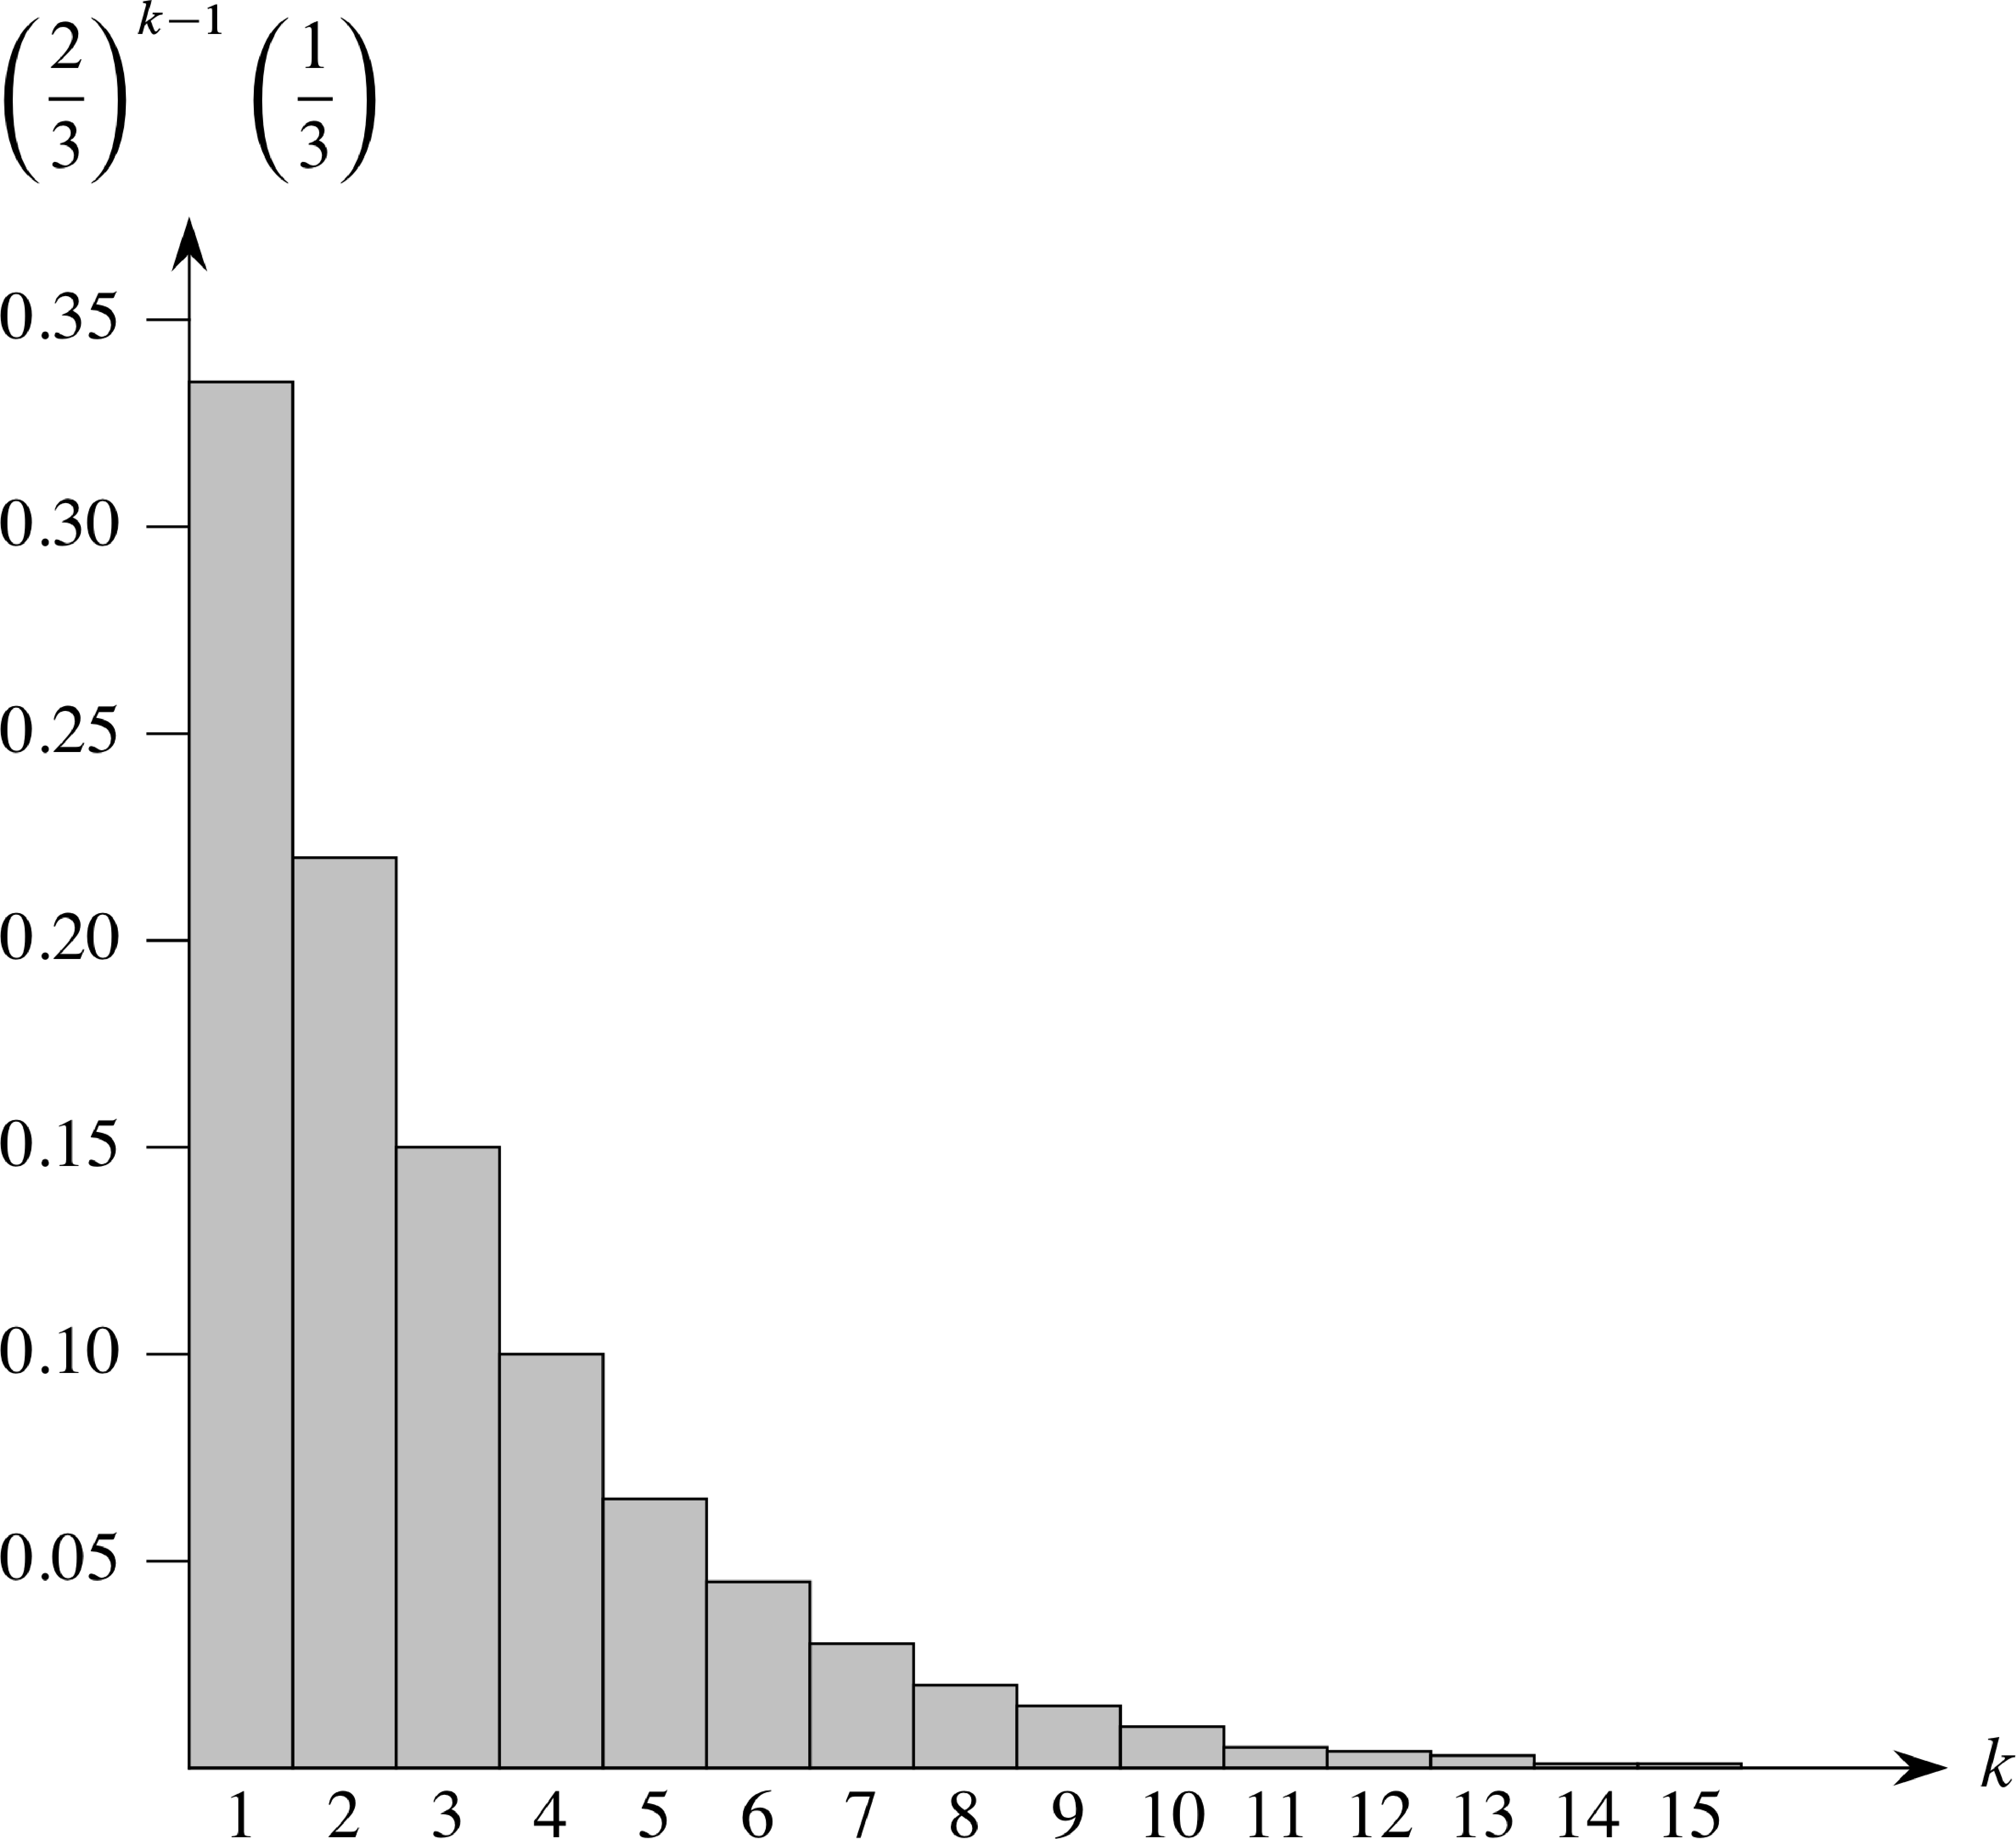
\includegraphics[height=.8\textheight]{Fig-C-1.pdf}


\end{frame}
\sect{Binomial distribution}
\bi
\item Probability of $k$ successes occur in $n$ Bernoulli trials with
   probability $p$:
  \[
  \pr{X=k} = {n\choose k}p^k(1-p)^{n-k}
  \]
\item We define a family of distributions:
  \[
  b(k:n,p) = {n\choose k}p^k(1-p)^{n-k}
  \]
  \ei
  
\end{frame}
\sect{Binomial distribution}
\vfill

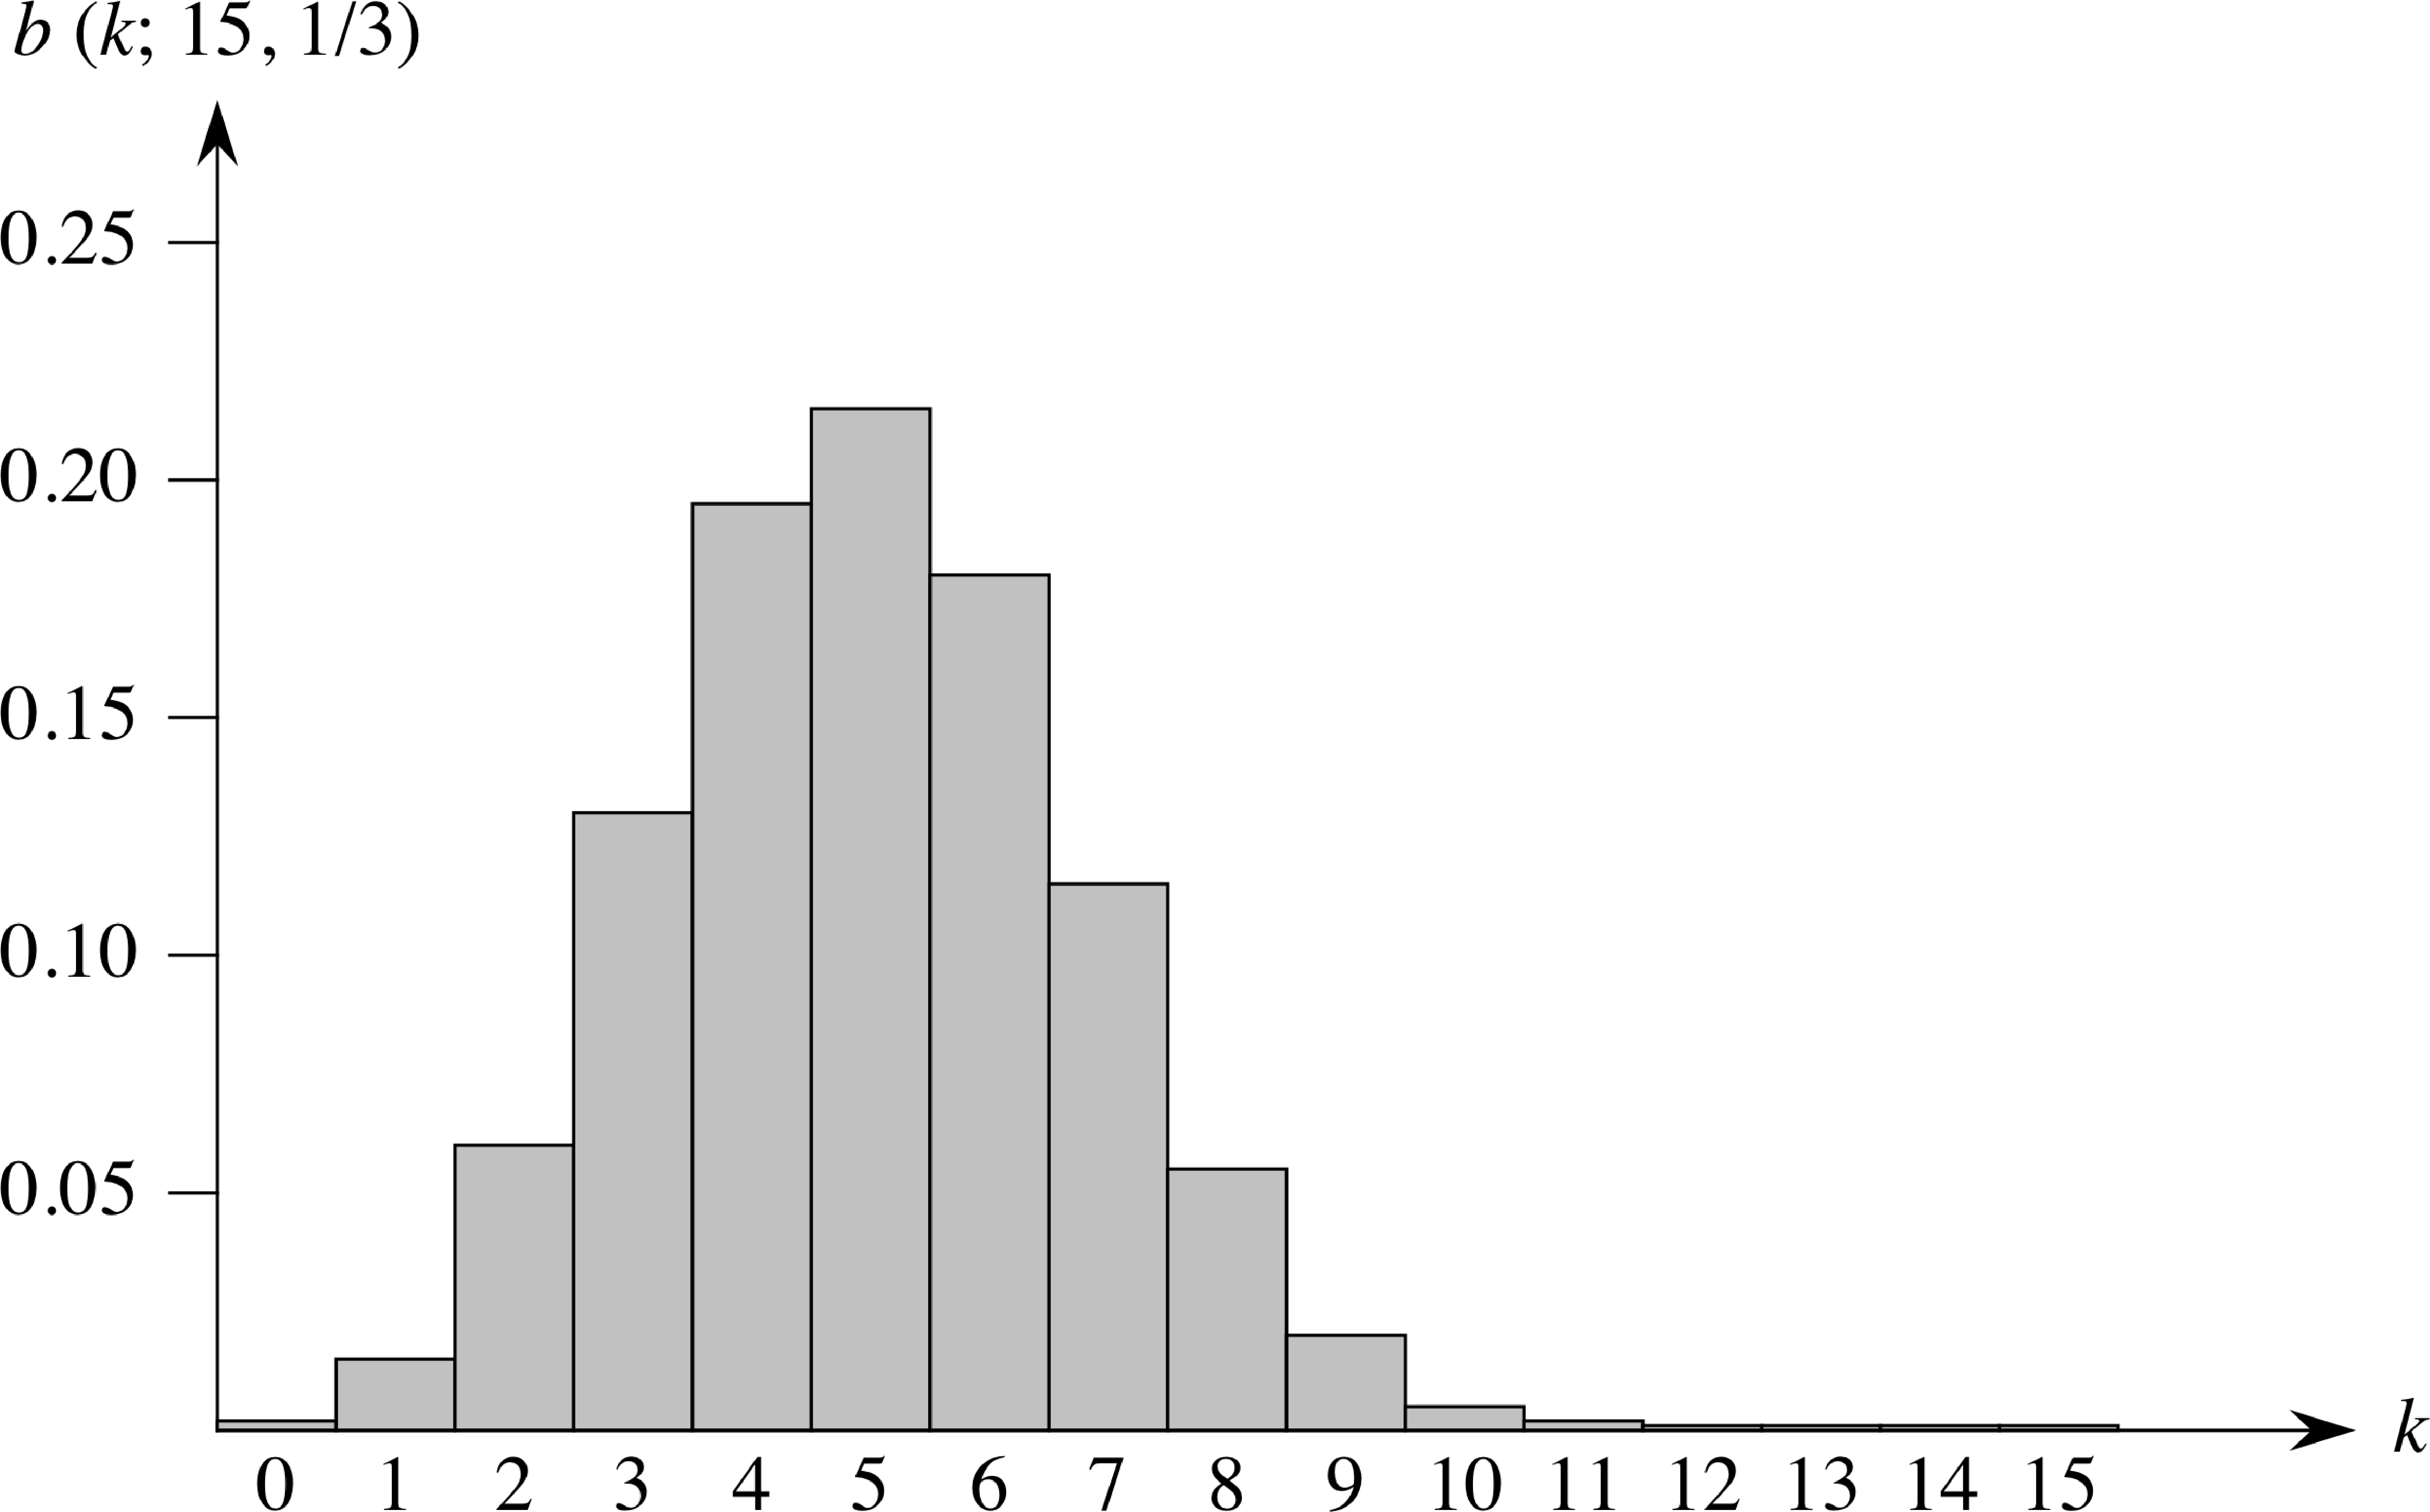
\includegraphics[width=\textwidth]{Fig-C-2.pdf}


\end{frame}
\sect{Binomial distribution expectation}
  \[
  \pr{X=k} = {n\choose k}p^k(1-p)^{n-k}
  \]
\bi
\item Expectation:
  \begin{align*}
    E[X] &= \sum_{k=0}^n k\cdot \pr{X=k}\\
    &= \sum_{k=0}^nk{n\choose k}p^kq^{n-k}\\ &= \mbox{\bf ?}
  \end{align*}
  \ei

\end{frame}
\sect{Binomial distribution expectation}
  \[
  \pr{X=k} = {n\choose k}p^k(1-p)^{n-k}
  \]
\bi
\item Let $X_i$ be an {\bf indicator random variable} for the $i$th trial.
\bi\item $X_i$ is 1 if the $i$th trial is a success, 0 otherwise.\ei
\item Easier math:
  \begin{align*}
    E[X] 
    &= E\left[\sum_{i=1}^{n} X_i\right]\\
    &= \sum_{i=1}^{n} E[X_i] & \mbox{linearity of expectation}\\
    &= \sum_{i=1}^{n} p = np
  \end{align*}

  \ei

\end{frame}
\sect{Binomial distribution variance}
  \[
  \pr{X=k} = {n\choose k}p^k(1-p)^{n-k}
  \]


\begin{align*}
  \mbox{Var}[X_i] &= E[X_i^2] - E^2[X_i]\\
  &=   E[X_i] - E^2[X_i]\\
  &= p - p^2 = pq
\end{align*}


\begin{align*}
  \mbox{Var}[X] 
  &= \mbox{Var}\left[\sum_{i=1}^{n} X_i\right]\\
&= \sum_{i=1}^{n} \mbox{Var}[X_i] \\
&= \sum_{i=1}^{n}  pq = npq
\end{align*}

\end{frame}

\sect{Binomial tails}
\begin{align*}
\pr{X\geq k} &= \sum_{i=k}^n b(i:n,p)\\
&\leq \binom{n}{k} p^k\\
\pr{X\leq k} &= \sum_{i=0}^k b(i:n,p)\\
&\leq \binom{n}{k} (1-p)^{n-k}
\end{align*}

\end{frame}


\end{document}
